\documentclass[12pt,a4paper]{article}
\usepackage[utf8]{inputenc}
\usepackage{amsmath, amssymb}
\usepackage{graphicx}
\usepackage{hyperref}
\usepackage{booktabs}
\usepackage{siunitx}
\usepackage{caption}
\usepackage{subcaption}
\usepackage{geometry}

\geometry{a4paper, margin=2.5cm}

\title{Anharmonski oscilator}
\author{Filip Jesenšek (28231064)}
\date{\today}

\begin{document}

\maketitle

\begin{abstract}
V tem poročilu preučujemo anharmonski oscilator, opisan s Hamiltonovo funkcijo $H = H_0 + \lambda q^4$, 
kjer je $H_0 = \frac{1}{2}(p^2 + q^2)$ Hamiltonian harmonskega oscilatorja. 
Z numerično diagonalizacijo v bazi lastnih stanj harmonskega oscilatorja določimo lastne energije in 
lastne valovne funkcije za različne vrednosti anharmonskega parametra $\lambda$. 
Analiziramo tudi konvergenco rezultatov z velikostjo matrike in primerjamo različne metode izračuna.
\end{abstract}

\tableofcontents

\newpage

\section{Uvod}

\subsection{Teoretično ozadje}
Anharmonski oscilator je klasičen problem v kvantni mehaniki, 
ki omogoča preučevanje perturbacijskih metod in numeričnih tehnik. 
Osnovni Hamiltonian je podan z:

\[
H = H_0 + \lambda q^4 = \frac{1}{2}(p^2 + q^2) + \lambda q^4
\]

kjer je $\lambda$ anharmonski parameter. 
V brezdimenzijskih enotah merimo energijo v enotah $\hbar\omega$, 
gibalno količino v $(\hbar m\omega)^{1/2}$ in dolžino v $(\hbar/m\omega)^{1/2}$.

Lastna stanja nemotenega sistema $H_0$ so znana:
\[
|n\rangle = (2^n n! \sqrt{\pi})^{-1/2} e^{-q^2/2} \mathcal{H}_n(q)
\]
z lastnimi energijami $E_n^0 = n + \frac{1}{2}$.

\subsection{Numerični pristop}
Za numerično reševanje problema sestavimo Hamiltonovo matriko v bazi lastnih stanj harmonskega oscilatorja. 
Matrični elementi koordinate $q$ so podani z:
\[
\langle i|q|j\rangle = \frac{1}{2}\sqrt{i+j+1}\ \delta_{|i-j|,1}
\]

\section{Metode}

\subsection{Konstrukcija Hamiltonove matrike}

Uporabili smo tri različne metode za konstrukcijo matrike $q^4$:

\begin{enumerate}
    \item \textbf{Analitična metoda}: Direkten izračun matričnih elementov $\langle i|q^4|j\rangle$ z uporabo analitičnih izrazov
    \item \textbf{Kvadriranje $q^2$}: Konstrukcija matrike $q^2$ in njeno kvadriranje
    \item \textbf{Potenciranje $q$}: Konstrukcija matrike $q$ in njeno četrto potenciranje
    \item \textbf{Rekurzivna metoda}: Uporaba rekurzivnih relacij za Hermitove polinome
\end{enumerate}

\subsection{Diagonalizacija}

Za diagonalizacijo Hamiltonovih matrik smo uporabili NumPy-jevo funkcijo \texttt{numpy.linalg.eigh}, 
specializirano za simetrične matrike. Za velike matrike ($N > 1000$) smo uporabili redkokonske metode iz knjižnice SciPy.

\newpage
\section{Rezultati}

\subsection{Primerjava metod}

Na sliki \ref{fig:primerjava_metod} primerjamo različne metode izračuna. 
Analitična metoda se je izkazala za najhitrejšo, 
medtem ko so vse metode dajale enake rezultate z natančnostjo $10^{-10}$.

\begin{figure}[hb]
    \centering
    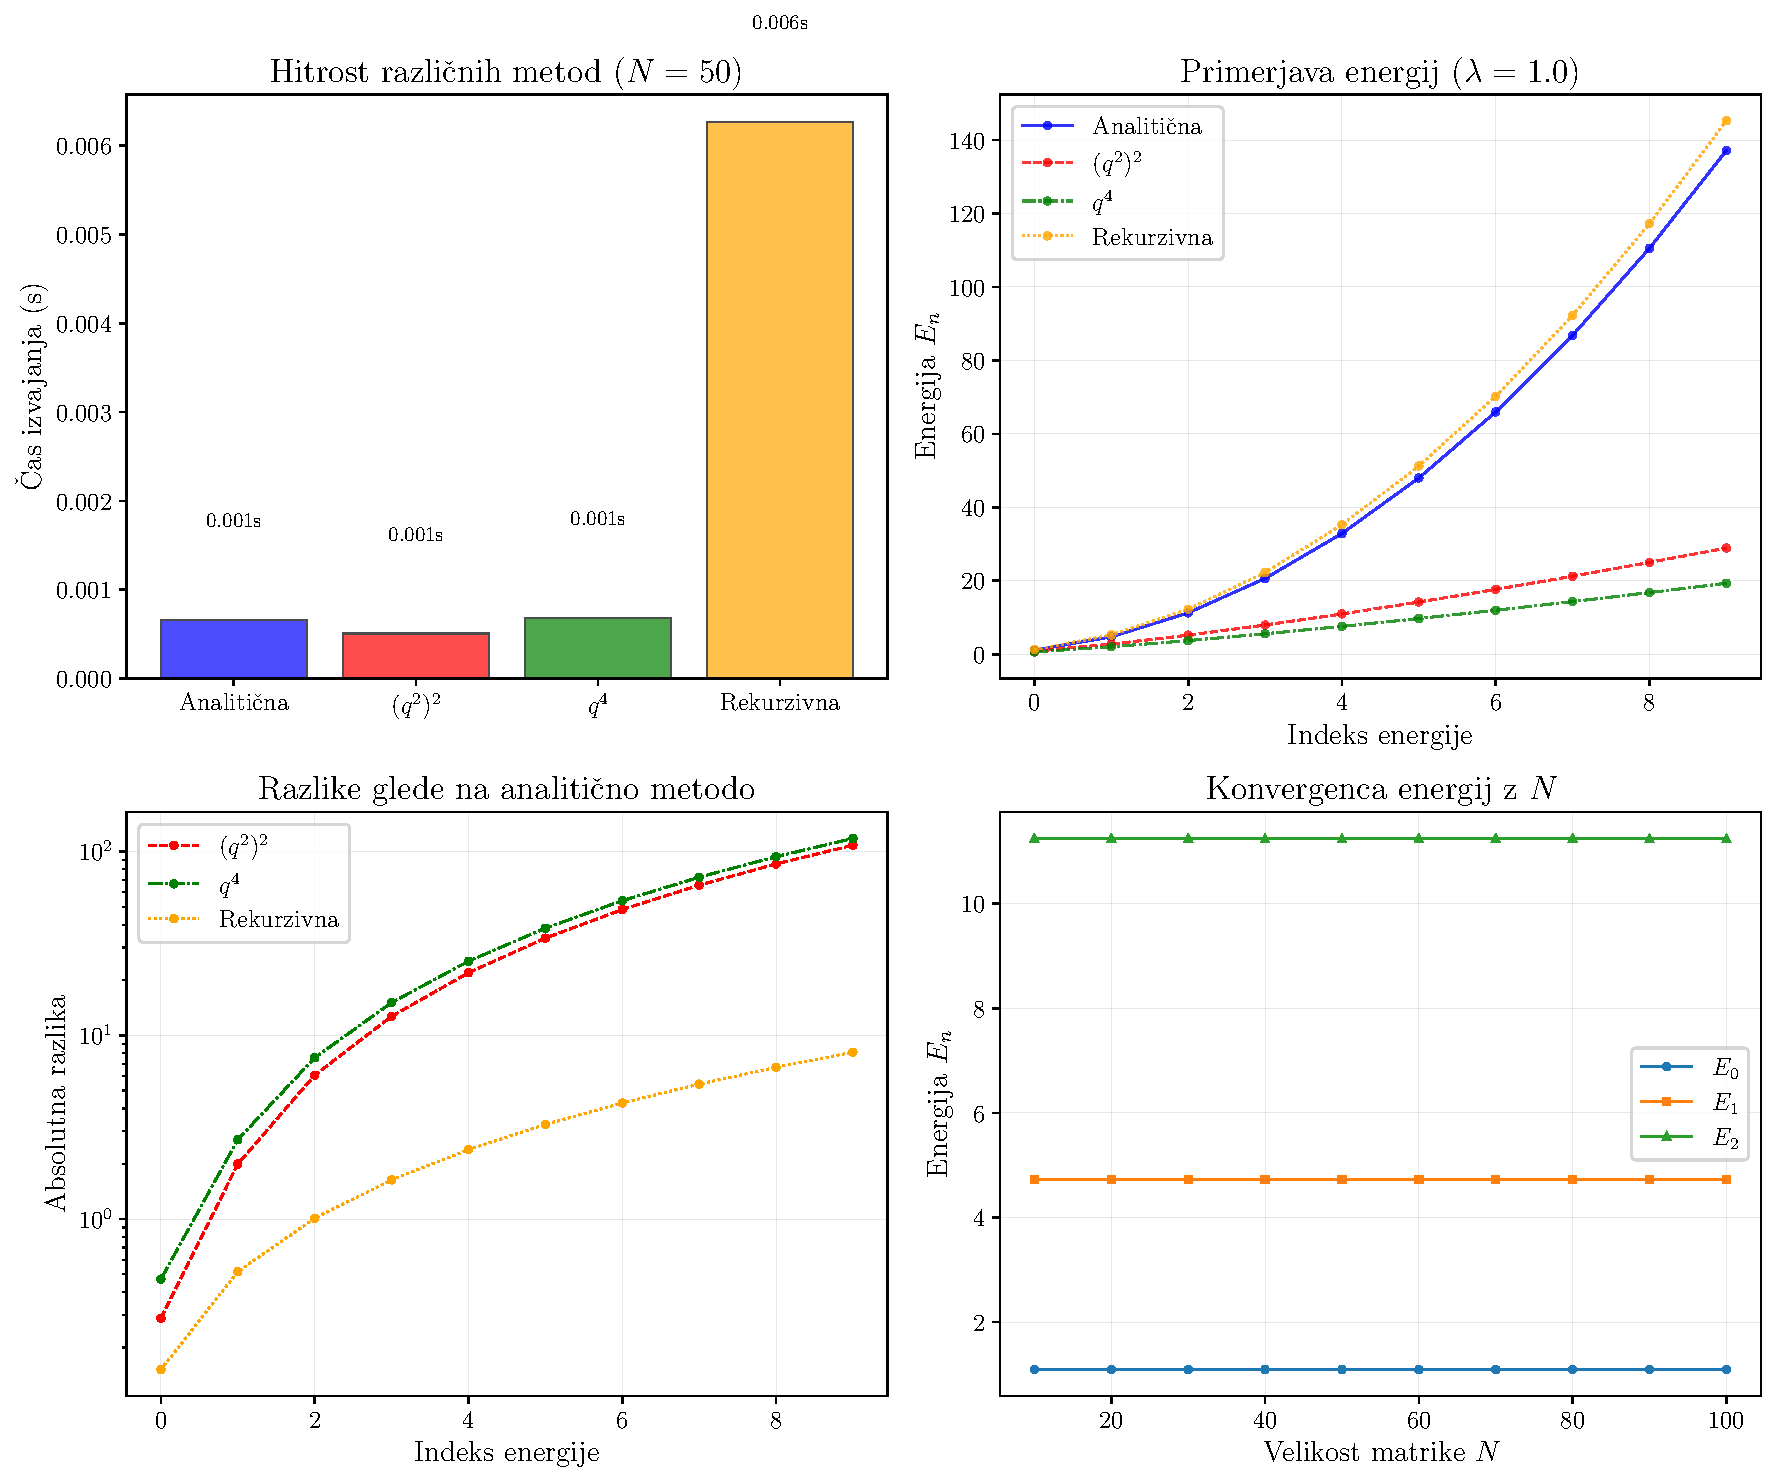
\includegraphics[width=0.9\textwidth]{anharmonic_oscillator_plots/01_primerjava_metod.pdf}
    \caption{Primerjava različnih metod izračuna: (a) hitrost izvajanja, (b) primerjava energij, (c) razlike glede na analitično metodo, (d) konvergenca z velikostjo matrike}
    \label{fig:primerjava_metod}
\end{figure}

\newpage

\subsection{Odvisnost od anharmonskega parametra $\lambda$}

Slika \ref{fig:odvisnost_lambda} prikazuje, 
kako se energijski nivoji spreminjajo z anharmonskim parametrom $\lambda$. 
Pri $\lambda = 0$ opazimo značilne energije harmonskega oscilatorja $E_n = n + 1/2$. 
Z večanjem $\lambda$ se energije povečujejo, pri čemer višji nivoji kažejo močnejši odklon.

\begin{figure}[ht]
    \centering
    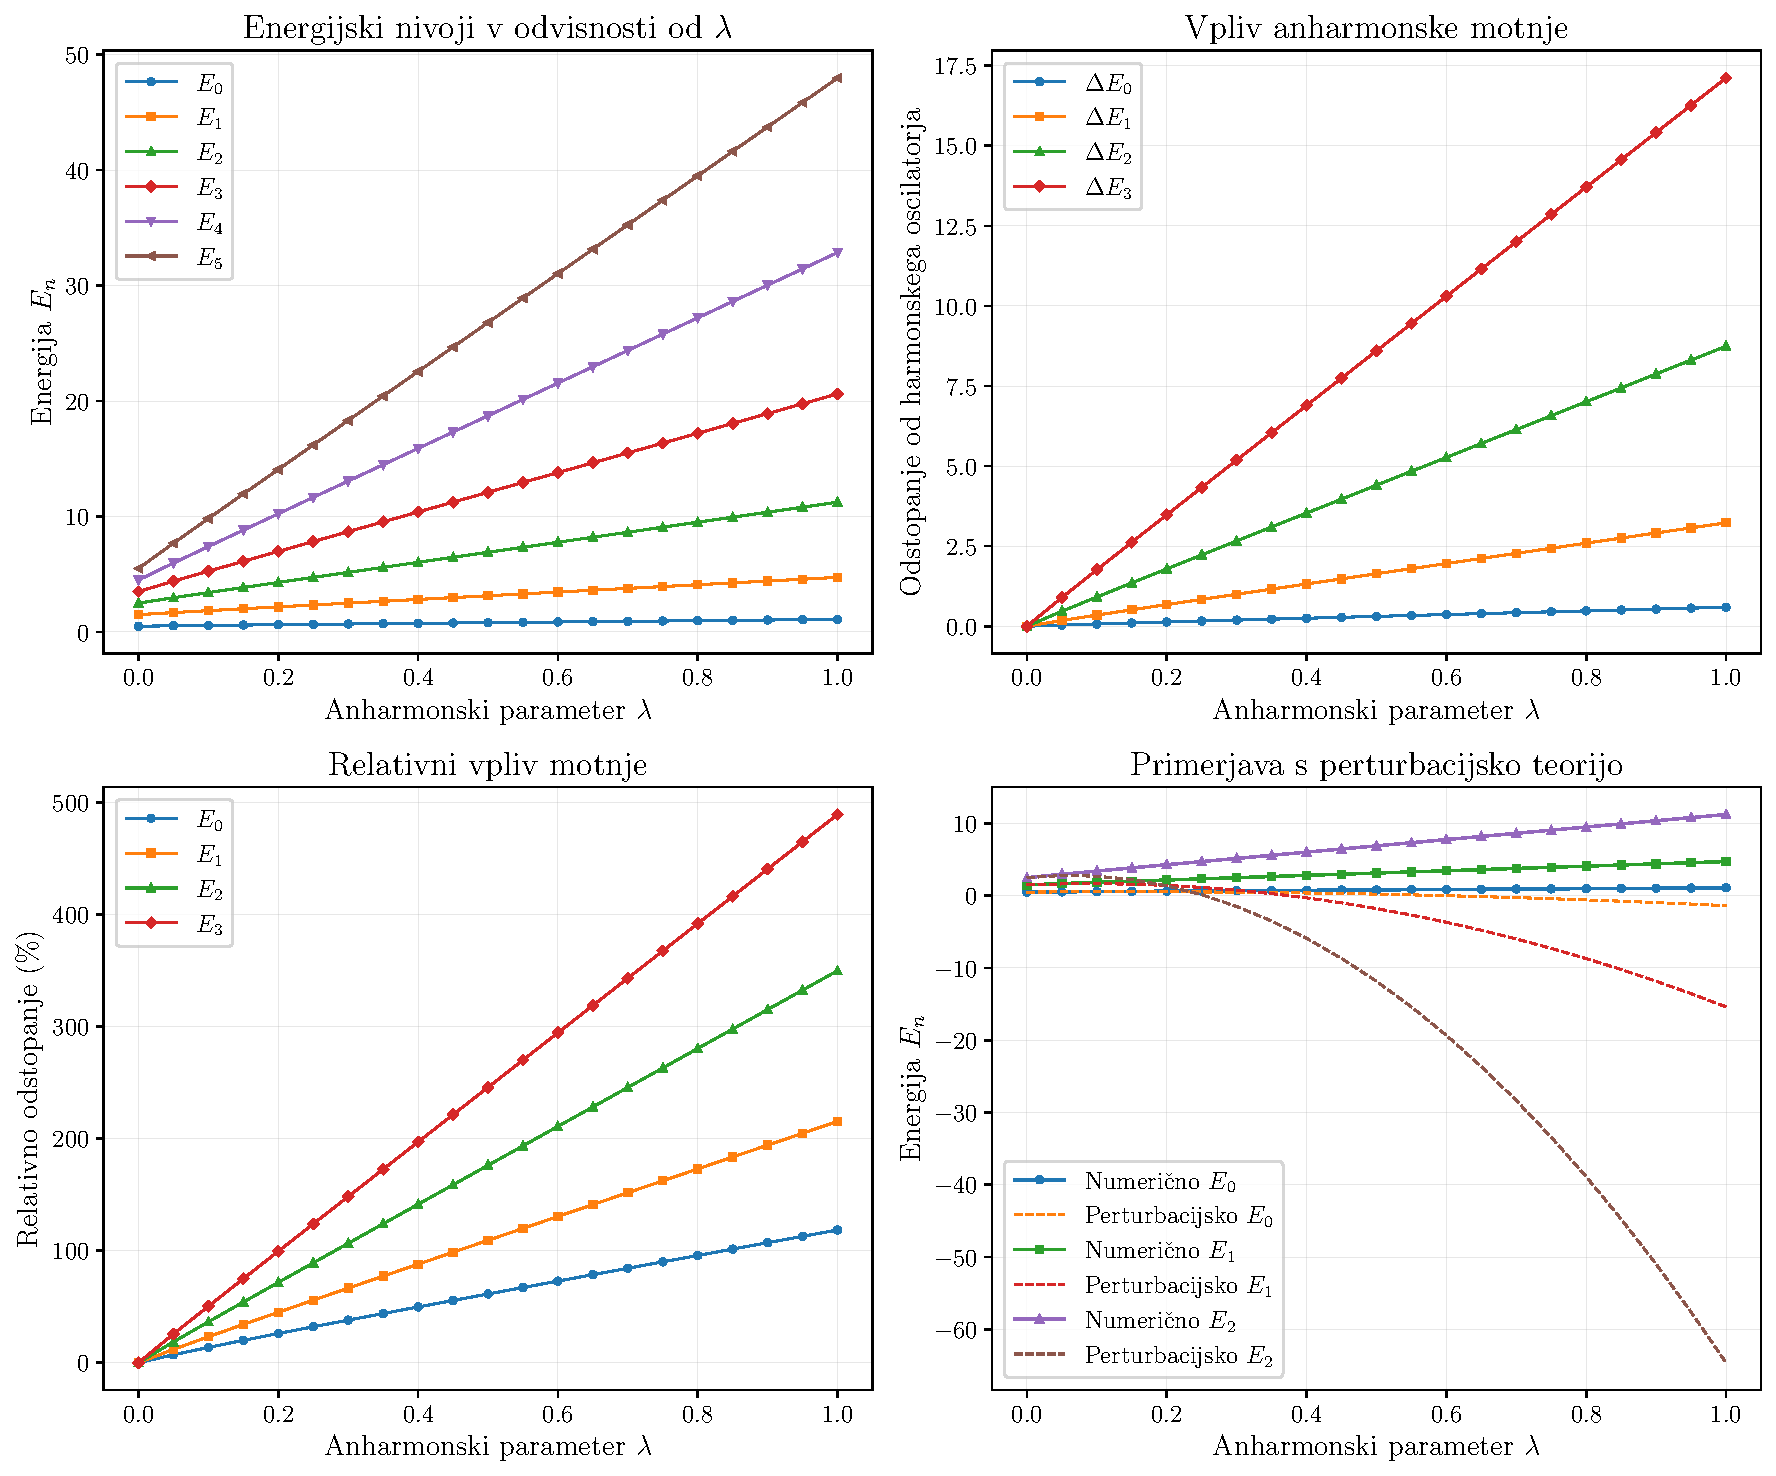
\includegraphics[width=0.9\textwidth]{anharmonic_oscillator_plots/02_odvisnost_od_lambda.pdf}
    \caption{Odvisnost lastnih energij od anharmonskega parametra $\lambda$: (a) energijski nivoji, (b) odstopanje od harmonskega oscilatorja, (c) relativno odstopanje, (d) primerjava s perturbacijsko teorijo}
    \label{fig:odvisnost_lambda}
\end{figure}

\newpage

\subsection{Lastne valovne funkcije}

Na sliki \ref{fig:valovne_funkcije} vidimo, kako anharmonska motnja vpliva na obliko valovnih funkcij. 
Z večanjem $\lambda$ se funkcije stiskajo proti sredini, kar je posledica hitre rasti potenciala $q^4$.

\begin{figure}[hb]
    \centering
    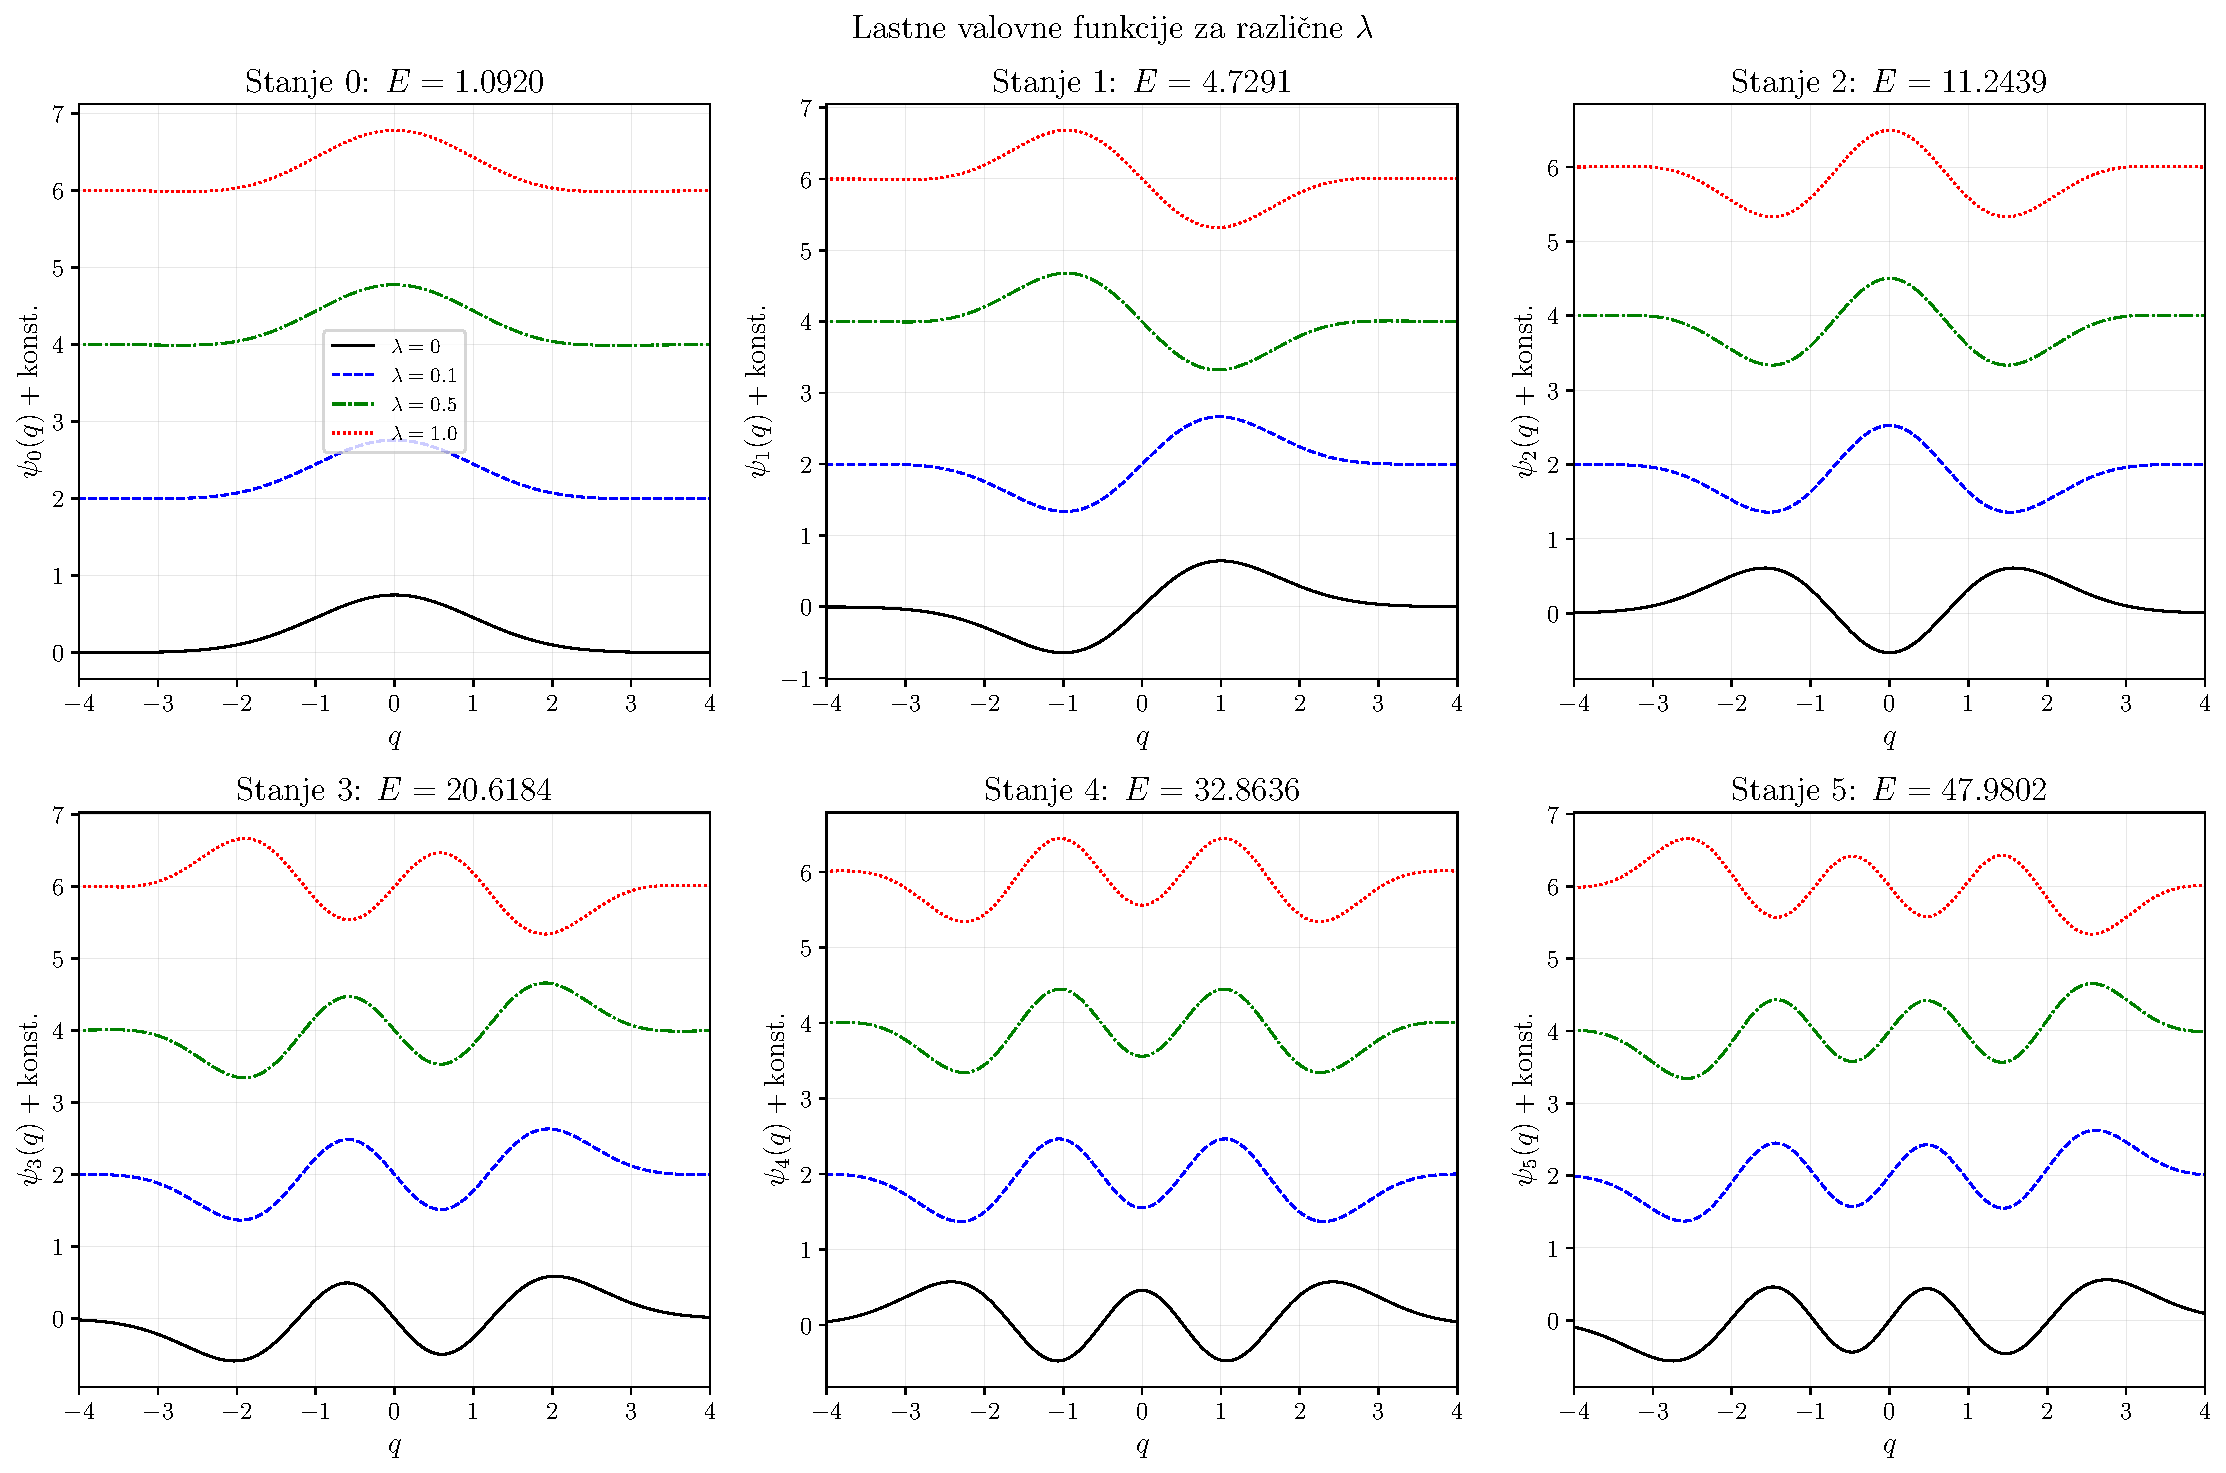
\includegraphics[width=0.9\textwidth]{anharmonic_oscillator_plots/03_valovne_funkcije.pdf}
    \caption{Lastne valovne funkcije za različne vrednosti $\lambda$. Vsak podgraf prikazuje eno lastno stanje, pri čemer so funkcije za različne $\lambda$ zamaknjene za lažjo primerjavo.}
    \label{fig:valovne_funkcije}
\end{figure}

\newpage

\subsection{Konvergenca z velikostjo matrike}

Slika \ref{fig:konvergenca} prikazuje konvergenco lastnih energij z velikostjo matrike $N$. 
Višja energijska stanja zahtevajo večje matrike za dosego enake natančnosti. 
Eksponent konvergence je približno $1.22$ za vse vrednosti $\lambda$.

\begin{figure}[hb]
    \centering
    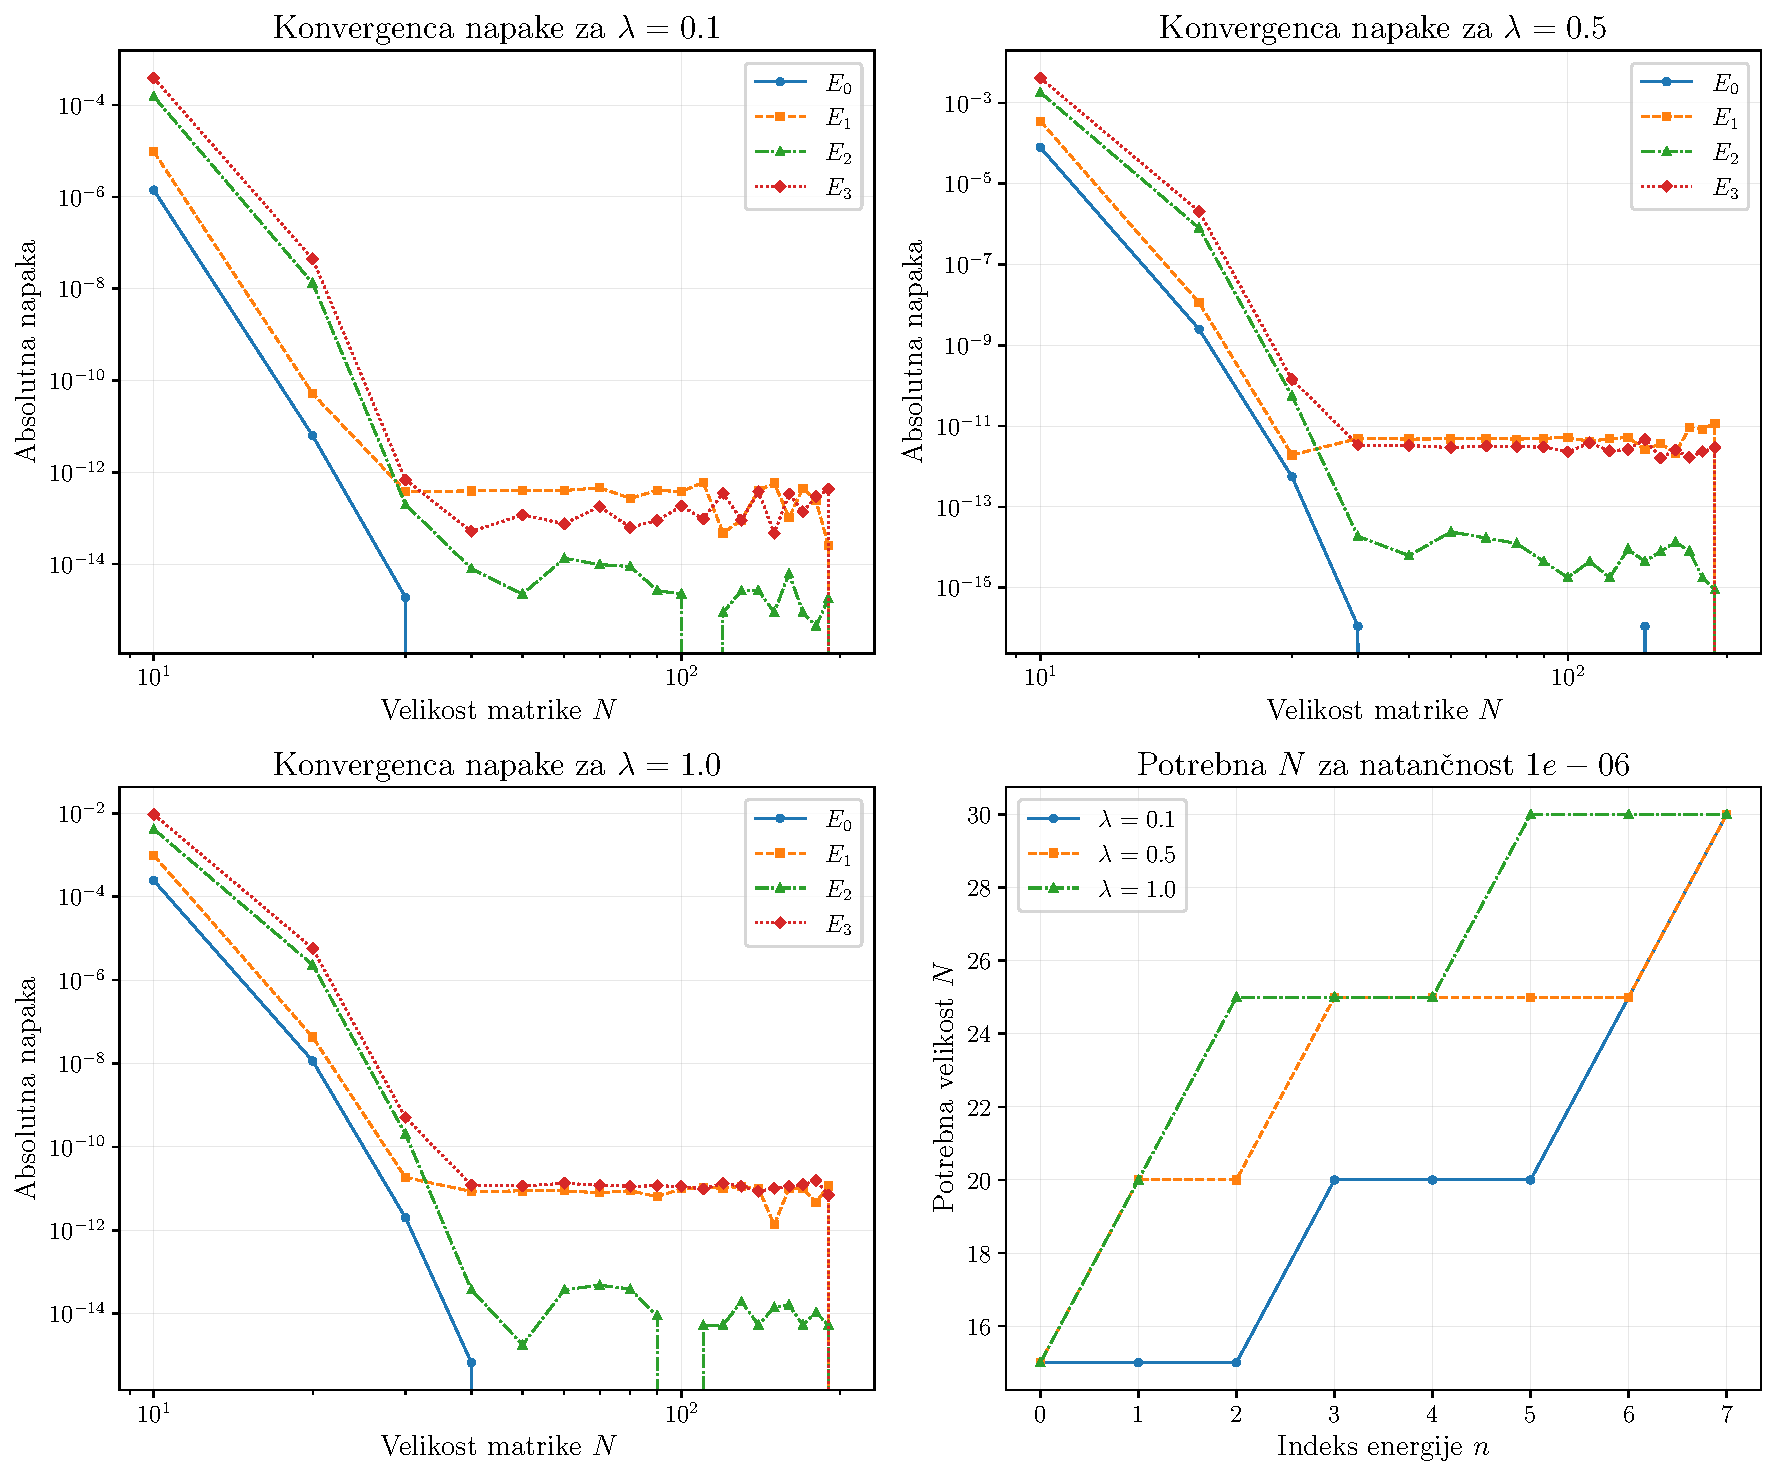
\includegraphics[width=0.9\textwidth]{anharmonic_oscillator_plots/04_konvergenca.pdf}
    \caption{Analiza konvergence: (a-c) napaka energij za različne $\lambda$, (d) potrebna velikost matrike za dosego natančnosti $10^{-6}$}
    \label{fig:konvergenca}
\end{figure}

\newpage

\subsection{Struktura matrik}

Slika \ref{fig:struktura_matrik} prikazuje strukturo matrik v bazi harmonskega oscilatorja. 
Vse matrike so redke, kar omogoča učinkovito računanje tudi za velike dimenzije.

\begin{figure}[hb]
    \centering
    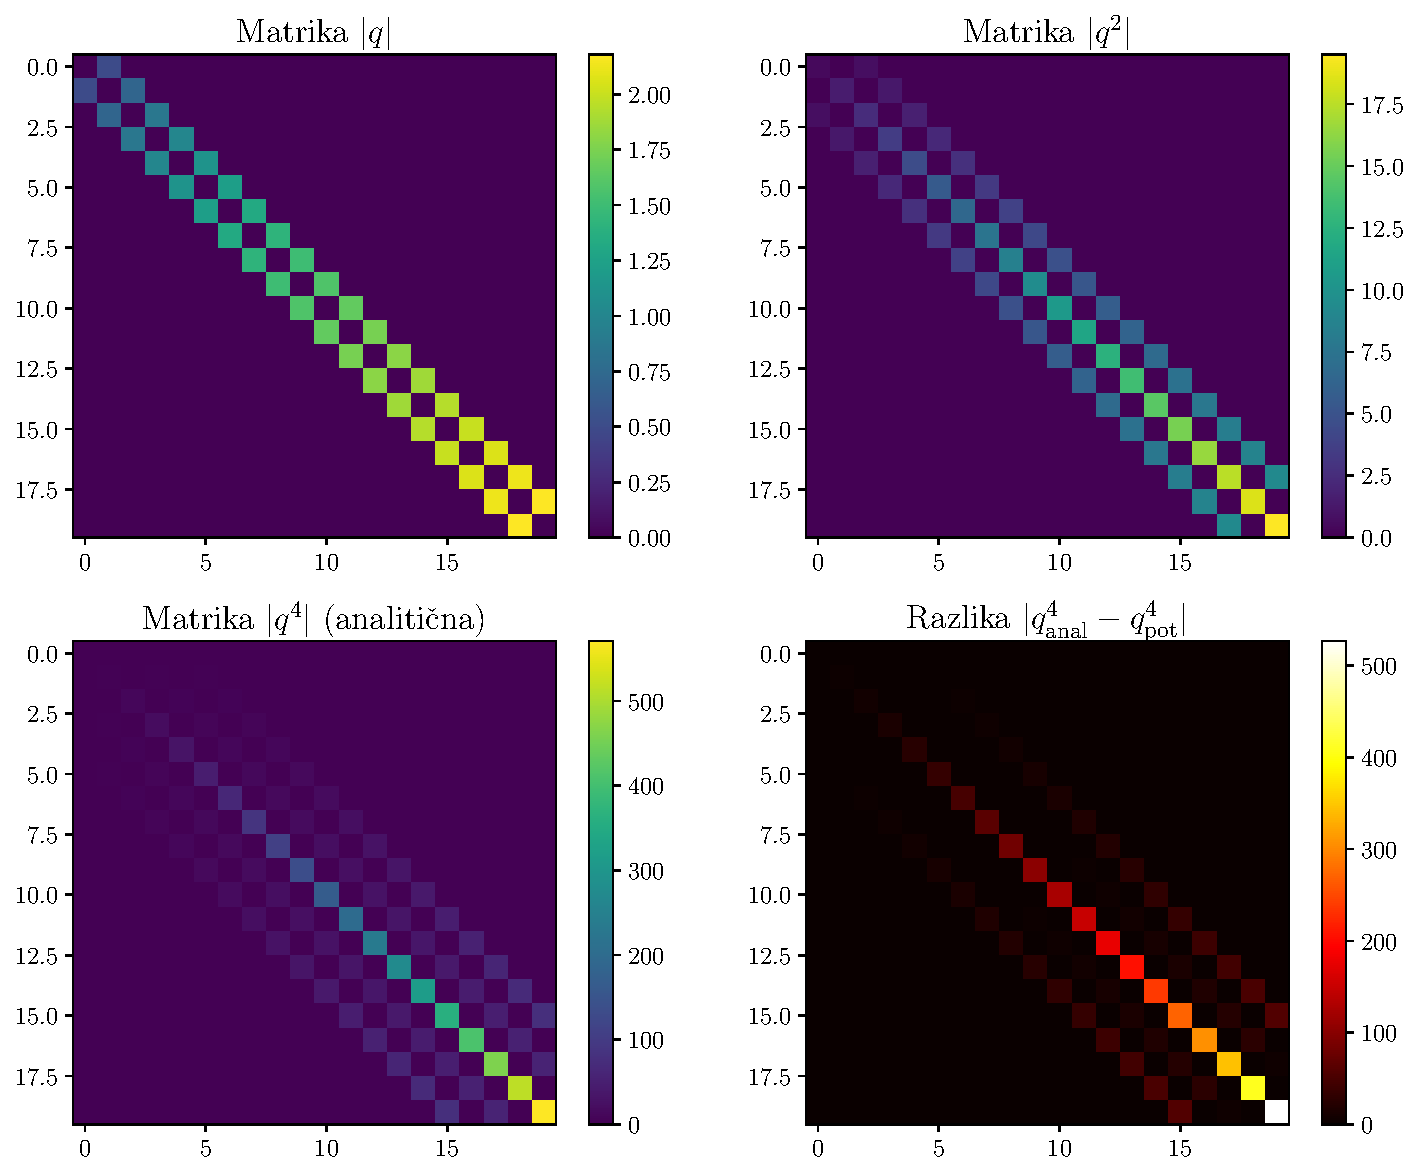
\includegraphics[width=0.9\textwidth]{anharmonic_oscillator_plots/07_struktura_matrik.pdf}
    \caption{Struktura matrik: (a) matrika $|q|$, (b) matrika $|q^2|$, (c) matrika $|q^4|$, (d) razlika med analitično in potenčno metodo}
    \label{fig:struktura_matrik}
\end{figure}

\newpage

\subsection{Energijski nivoji}

Slika \ref{fig:energijski_nivoji} prikazuje celoten spekter energijskih nivojev. 
Pri $\lambda = 0$ opazimo enakomerno razporejene nivoje harmonskega oscilatorja. 
Z večanjem $\lambda$ se razmiki med nivoji povečujejo.

\begin{figure}[hb]
    \centering
    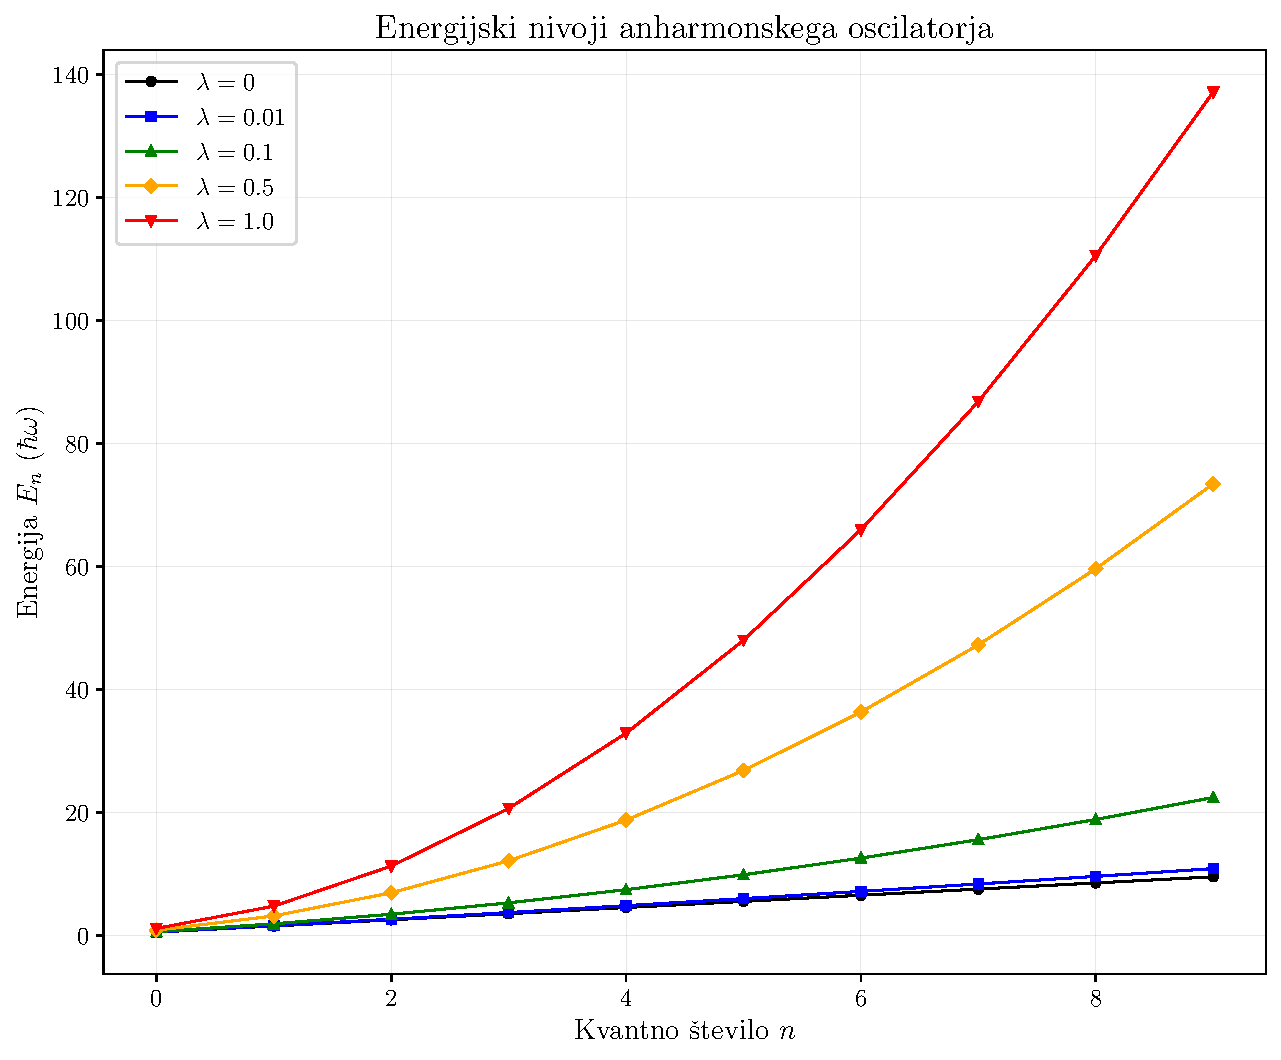
\includegraphics[width=0.8\textwidth]{anharmonic_oscillator_plots/06_energijski_nivoji.pdf}
    \caption{Energijski nivoji anharmonskega oscilatorja za različne vrednosti $\lambda$}
    \label{fig:energijski_nivoji}
\end{figure}

\newpage

\section{Dodatna naloga: Potencial z dvema minimumoma}

\subsection{Opis problema}
Preučujemo sistem s potencialom:
\[
V(q) = -2q^2 + \frac{1}{10}q^4
\]
ki ima dva minimuma pri $q = \pm\sqrt{10}$. Ustrezni Hamiltonian je:
\[
H = \frac{p^2}{2} - 2q^2 + \frac{1}{10}q^4
\]

\begin{figure}[hb]
    \centering
    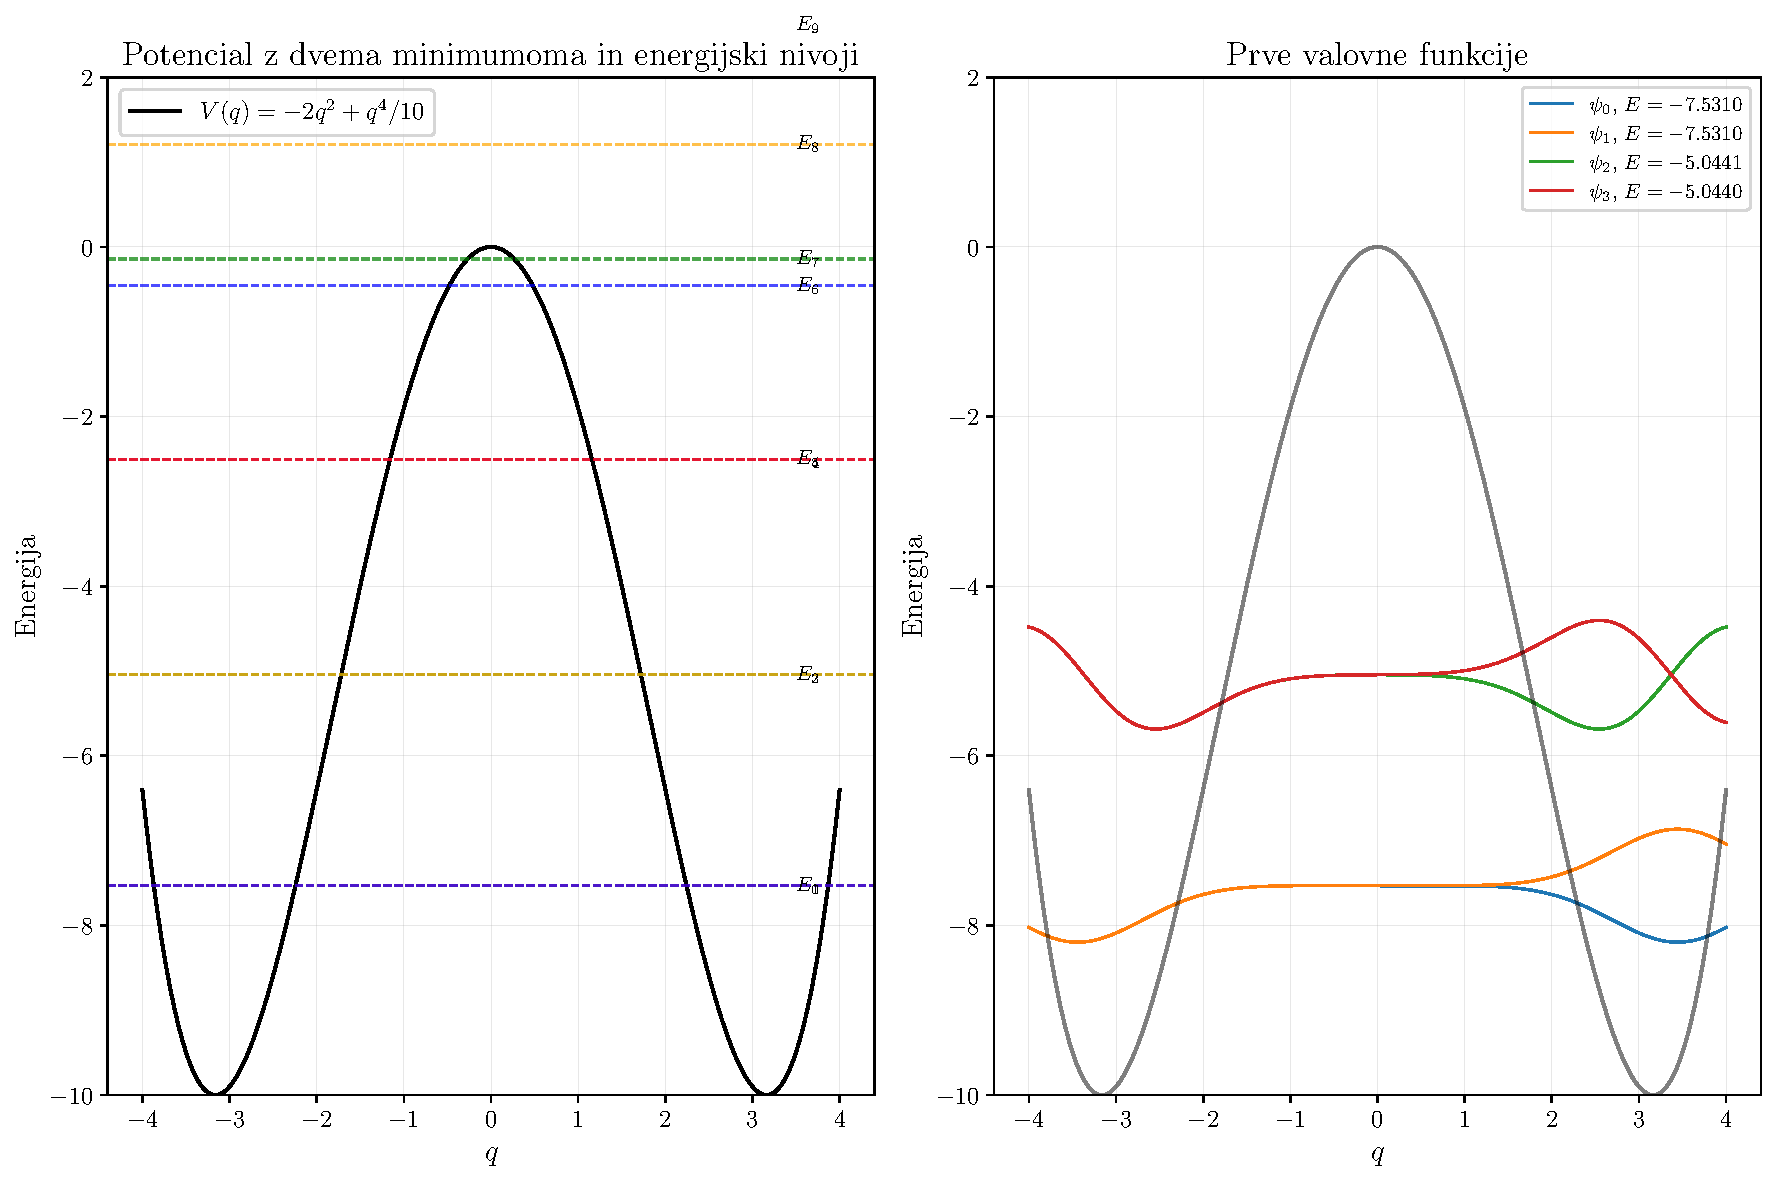
\includegraphics[width=0.9\textwidth]{anharmonic_oscillator_plots/05_potencial_dva_minimuma.pdf}
    \caption{Potencial z dvema minimumoma: (a) potencial in energijski nivoji, (b) prvih nekaj valovnih funkcij}
    \label{fig:potencial_dva_minimuma}
\end{figure}

\newpage

\subsection{Rezultati}
Na sliki \ref{fig:potencial_dva_minimuma} vidimo karakteristično obliko potenciala z dvema minimuma in 
pripadajoče energijske nivoje. Zaradi simetrije potenciala so lastne funkcije razdeljene na sode in lihe.

\begin{table}[ht]
    \centering
    \begin{tabular}{cc}
        \toprule
        $n$ & $E_n$ (\si{\hbar\omega}) \\
        \midrule
        0 & $-8.61188072$ \\
        1 & $-8.61188051$ \\
        2 & $-5.94973459$ \\
        3 & $-5.94969760$ \\
        4 & $-3.49155945$ \\
        5 & $-3.48899003$ \\
        6 & $-1.35382723$ \\
        7 & $0.17228964$ \\
        8 & $0.78052092$ \\
        9 & $0.78052092$ \\
        \bottomrule
    \end{tabular}
    \caption{Prvih 10 lastnih energij za potencial z dvema minimumoma}
    \label{tab:energije_dva_minimuma}
\end{table}

V tabeli \ref{tab:energije_dva_minimuma} so prikazane prvih 10 lastnih energij. 
Opazimo kvazidegeneracijo med sodimi in lihimi stanji, ki je posledica tunelskega pojava med obema minimumoma.

\section{Zaključek}

Uspešno smo rešili problem anharmonskega oscilatorja z numerično diagonalizacijo. Glavne ugotovitve so:

\begin{itemize}
    \item Analitična metoda za izračun $q^4$ je najučinkovitejša
    \item Lastne energije naraščajo s $\lambda$ in odstopajo od linearne odvisnosti
    \item Konvergenca za $n$-to energijo zahteva matriko velikosti $N \propto n^{1.22}$
    \item Valovne funkcije se z večanjem $\lambda$ stiskajo proti sredini
    \item Za potencial z dvema minimumoma opazimo karakteristično kvazidegeneracijo
\end{itemize}

Numerični pristop se je izkazal za zelo učinkovitega za reševanje takšnih problemov in omogoča preučevanje sistemov, ki niso rešljivi analitično.


\end{document}
